\documentclass[conference]{IEEEtran}
%\IEEEoverridecommandlockouts
% The preceding line is only needed to identify funding in the first footnote. If that is unneeded, please comment it out.
\usepackage{cite}
\usepackage{amsmath,amssymb,amsfonts}
\usepackage{algorithmic}
\usepackage[bottom]{footmisc}
\usepackage{graphicx}
\usepackage{textcomp}
\usepackage{xcolor}
\def\BibTeX{{\rm B\kern-.05em{\sc i\kern-.025em b}\kern-.08em
    T\kern-.1667em\lower.7ex\hbox{E}\kern-.125emX}}
\begin{document}

\title{Chapter X Section Y: Internet Routing Security}

\maketitle

\begin{abstract}
This chapter introduces the weaknesses of Internet routing and how they can be addressed in practice.
\end{abstract}

\section{Introduction}
Imagine you are listening to a playlist on Youtube and the music suddenly stops.  It seems like you still have access to other websites, so this must be a technical problem at Youtube, right?  Back in 2008, something similar happened to people across the globe, but it had nothing to do with technical issues at Youtube.  Instead, the state run network of Pakistan caused all Youtube traffic to be diverted into the network equivalent of a black hole.  It turned out that Pakistan was simply trying to block Youtube for users within its borders, and yet it still managed to take Youtube down for almost all users across the world.  How could a network in Pakistan cause users in Boston to be unable to reach services hosted in California?  And if this is possible, couldn't this same technique be used by cyber criminals to steal sensitive information?  In this section, we will address how this is possible and what can be done to mitigate it.

\section{Internet Routing: Address and Number Assignment}
\begin{figure}
  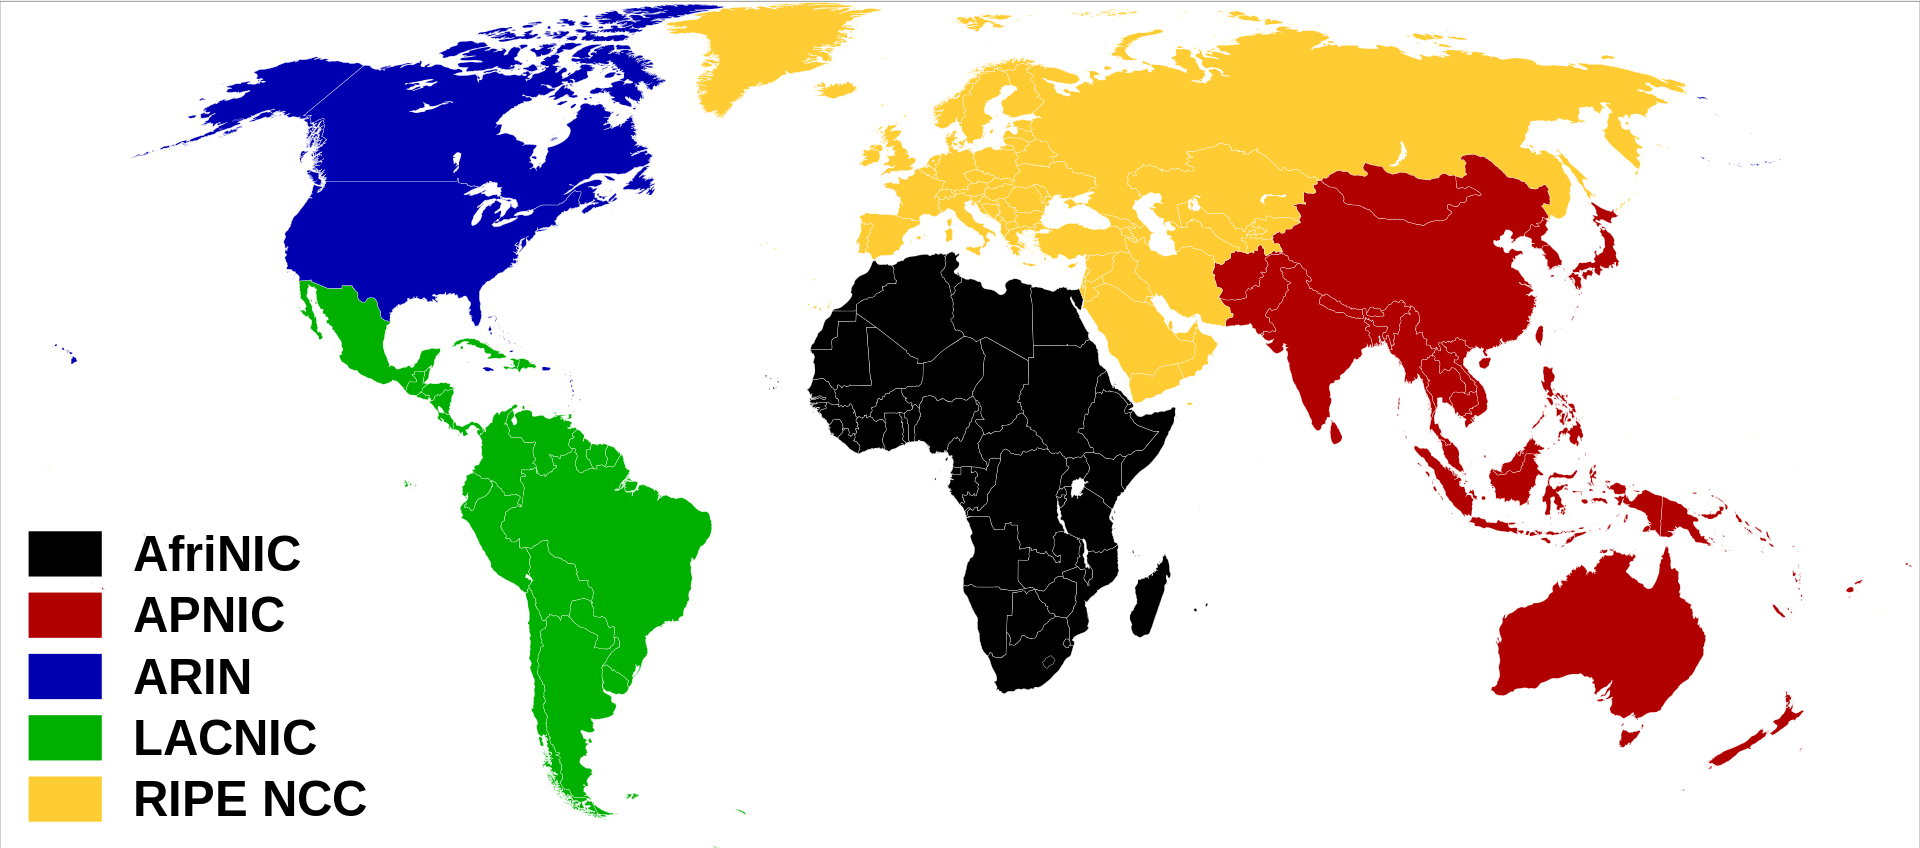
\includegraphics[width=\linewidth]{images/rirs.png}
  \caption{Regional Internet Registries manage the IP block assignment and Autonomous Systsem Number assignment for geographically local areas.}
  \label{fig:rirs}
\end{figure}

Before one can understand the weaknesses of Internet routing, one must understand how the Internet routing system is intended to work.  Individuals and organizations rely on Internet Service Providers (ISPs) to direct their network traffic to the appropriate destinations.  Any organization that wants to connect to the Internet must be given an IP address from an ISP or a block of IP addresses from a regional organization that manages IP address assignments known as a Regional Internet Registry (RIR).  Figure \ref{fig:rirs} shows examples of RIRs and the regions which they manage the IP space for.  Oragnizations that that want a set of their own IP addresses must also be assigned an Autonomous System Number (ASN).  ASNs are unique numbers which identify an organization's network in the global Internet.  It is common for a network to be assigned a single ASN and one or many contiguous blocks of IP addresses, as seen in Figure \ref{fig:rir-assignments}.

\begin{figure}
  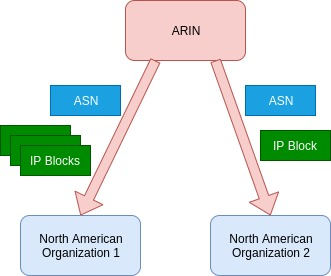
\includegraphics[width=\linewidth]{images/rir-assignments.jpg}
  \caption{Regional Internet Registries often assign a single ASN for each organization.  They also often assign one or many contiguous IP blocks to those organizations.}
  \label{fig:rir-assignments}
\end{figure}

\section{Internet Routing Operation}
In order to reach a service like Youtube, users need to know how to reach the service.  Youtube may have a set of IP addresses to allow users to connect to, but there are still two technical challenges:
\begin{enumerate}
 \item Youtube needs to announce where those IP addresses exist in the Internet
 \item The Internet itself needs to announce the path to take in order to get there to potential users
\end{enumerate}
The Border Gateway Protocol (BGP) is used to solve these problems, and its operations are illustrated in Figure \ref{fig:bgp-ops}.  The organization that owns the IP addresses announces those addresses as an IP prefix \footnote{An IP prefix could be one of the blocks assigned to the organization, or it could be a contiguous subset of IP addresses within that block.} into its upstream ISP, which takes care of challenge 1.  In that same announcement, Youtube also announces its ASN.  When Youtube's ISP connects to another network, it appends its own ASN to the list.  This process continues throughout the Internet, allowing for each network to know which path or paths it can take to reach Youtube.  These paths, known as AS paths, should all begin with Youtube's ASN, which effectively acts as a mapping between Youtube and the IP space in the global Internet.  These AS paths are used to address challenge 2.

If there are multiple paths to a target IP address, BGP uses a decision process similar to that in Figure \ref{fig:bgp-dec} \footnote{The BGP decision process is not standardized, and it may vary across different implementations.  Many implementations are very similar.}.  One of the most critical steps in the decision process, especially in the ISPs BGP decision making, is the AS path length.  It is often the case that the path with the shortest AS path length is the preferred route for traffic to a destination with a given IP address.

\begin{figure}
  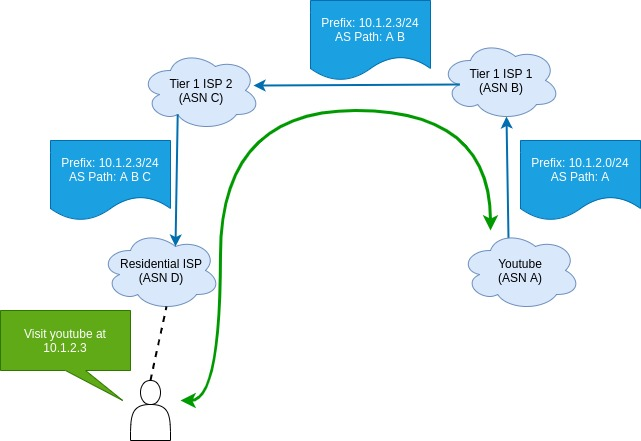
\includegraphics[width=\linewidth]{images/bgp-ops.jpg}
  \caption{The Border Gateway Protocol is used to announce the source of IP prefixes into the global Internet and to create paths from other organization's networks to those IP addresses.}
  \label{fig:bgp-ops}
\end{figure}

FIXME: need figure showing BGP decision process

\section{BGP Hijacking}
With an understanding of how BGP operates, it is now useful to revisit the case of Youtube and the state run network of Pakistan.  What happened was Pakistan's state run network attempted to take all traffic destined for IP addresses in Youtube's IP prefixes and send them to a place in its own internal network that connected to nothing.  By mistake, this change in their internal network was announced, via BGP, to the rest of the world.  Figure {fig:bgp-hijack} illustrates what may have happened for some users who experienced a Youtube outage.  This problem is known as BGP Hijacking, and this example illustrates that the BGP has an inherent weakness: the receiver of the BGP announcement trusts the sender of the announcement, who in turn trusted the sender of the previous BGP announcement, and so on.  This trust model is known as "transitive trust", and it is part of why BGP scales well and part of why BGP is not secure.  BGP Hijacking can be unintentional, such as the Youtube example, but it can also be weaponized by others with malicious intent for data interception or denial of service.  This is why it is so important that mitigation techniques be deployed across the Internet to avoid this weakness.

\begin{figure}
  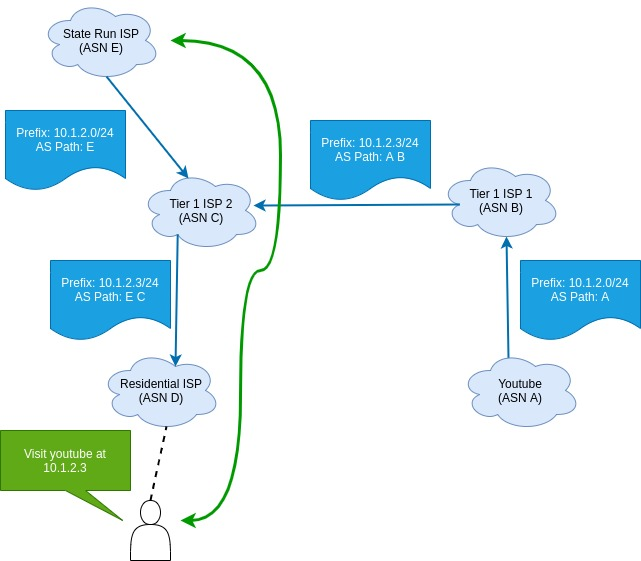
\includegraphics[width=\linewidth]{images/bgp-hijack.jpg}
  \caption{The state run network of Pakistan announced ownership of Youtube's IP prefixes to the rest of the world.  For many users, this ended up being the shortest AS path between them and Youtube.}
  \label{fig:bgp-hijack}
\end{figure}

\section{BGP Hijacking Mitigation Techniques}
There are various techniques which can me used to mitigate the weaknesses in BGP.

\subsection{Filtering}

\subsection{Resource Public Key Infrastructure}

\subsection{BGPsec}

\end{document}
